\chapter{PROSPECT}

The scientific community's understanding of neutrinos has come a long way from Pauli's initial proposition of its existence in 1930. 
Though three active neutrino flavors and their behaviors are understood and well included in the Standard Model of particle physics, recent anomalies in reactor neutrino experiment results hint at the possibility of new physics. 
The discovery of an eV-scale sterile neutrino would have wide ranging impacts on the field of neutrino physics and future experiments.

The Precision Reactor Oscillation and Spectrum Experiment (PROSPECT) is designed to address the reactor antineutrino anomaly by performing a reactor-model independent search for short-baseline $\bar{\nu_{e}}$ oscillations and making a high precise measurement of the $^{235}$U $\bar{\nu_{e}}$ energy spectrum at a highly-enriched uranium (HEU) research reactor \cite{LongNIM}.
Located at the High Flux Isotope Reactor (HFIR) at Oak Ridge National Laboratory (ORNL) in Tennessee PROSPECT also demonstrates successful application of techniques for antineutrino detection at the surface with little overburden. 
PROSPECT collected data from May to December of 2018 and the first oscillation and spectrum results, with 33 and 40.3 live-days of reactor on time respectively, can be found in Ref.\cite{PhysRevLett.121.251802,Ashenfelter:2018jrx}.

\section{Experimental Site}
\subsection{HFIR}

HFIR is a compact research reactor that burns highly enriched uranium fuel ($^{235}$U), meaning that $>$ 99\% of fissions during a reactor cycle will be from $^{235}$U.
The HFIR core consists of two concentric fuel elements with an outer diameter of 0.435 m and a height of 0.508 m, surrounded by control elements and Beryllium reflectors as shown in Figure~\ref{fig:hfir}. 
The reactor typically operates at 85 MW for seven 24-day cycles per year for a duty cycle of $\sim$46\%.

\begin{figure}[t]
	\centering
	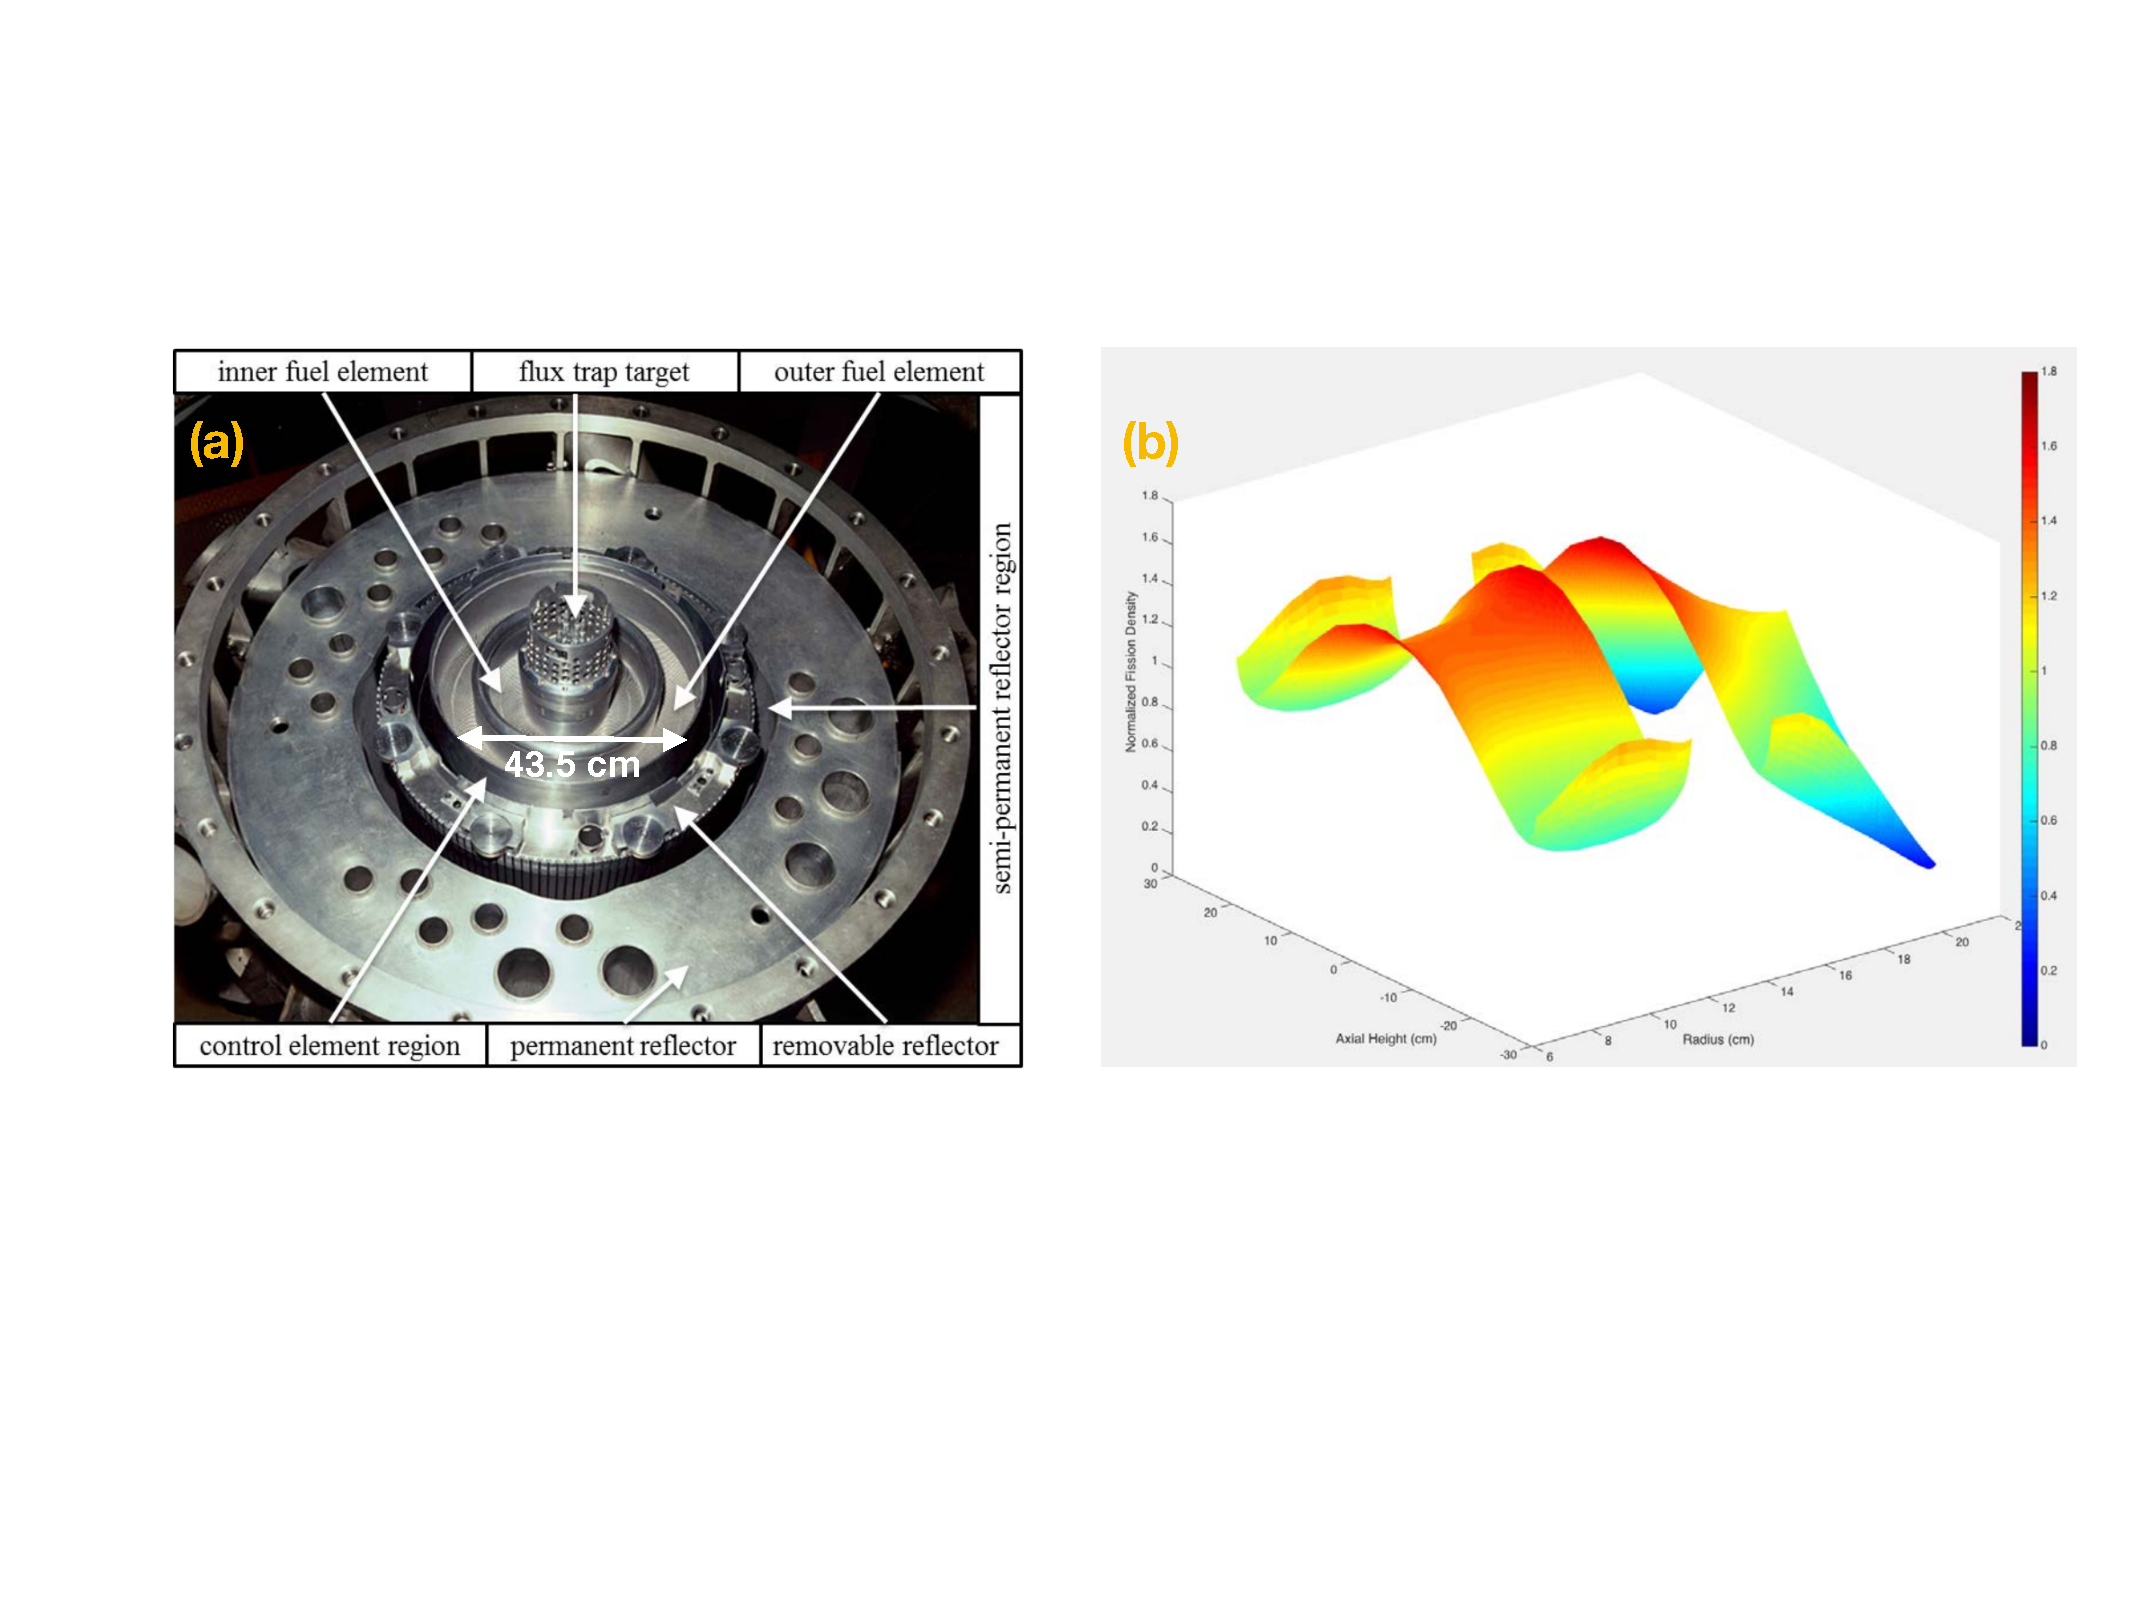
\includegraphics[width=0.9\linewidth]{tex/4-prospect-images/HFIR}
	\caption[The HFIR core and flux distribution]{(a) The HFIR core, showing the inner and outer fuel elements and the flux trap region, as well as the control elements and Beryllium reflectors. (b) The relative fission density distribution at the start of a cycle. \cite{HFIRTech}}
	\label{fig:hfir}
\end{figure}

\subsection{Backgrounds at HFIR}

The PROSPECT detector is located at ground level $\sim$7 m from the HFIR core and separated from the reactor water pool by a 1 m thick concrete wall, show in Figure~\ref{fig:shielding}.
The proximity to the reactor and lack of overburden introduces a significant level of background events from the reactor and cosmogenic sources. 
These events can be classified into two categories, (i) singles that are mainly due to gammas and (ii) coincident events from neutron recoil and captures. 
Extensive studies on the types and rate of background events at the detector site can be found in Refs.\cite{Ashenfelter:2015tpm,Heffron,Hackett}.

The largest source of gamma backgrounds was discovered to originate in the reactor pool wall, specifically an unused beam line that lies directly in front of the detector. 
In order to lower these backgrounds a lead shield wall (3.0 m wide, 2.1 m tall, and on average 0.10 m thick), along with shorter flanking walls on each side and a mini-wall placed at the opening of the beam line, was installed between the pool wall and the detector.
Other background events were shown to come from neutron beam-lines and scattering experiments existing below the detector site, but most of these are suppressed by a concrete monolith that the detector sits on.

The thermal neutron rate was measured to be $\sim$2/cm$^2$/s during reactor operation \cite{Ashenfelter:2015tpm}, so layers of shielding containing $^{10}$B, which has a large thermal neutron cross-section and minimal gamma emission, were used in the passive shielding that surrounds the detector (see Section~\ref{sec:shielding}). 
The locally installed shield wall, along with the addition of passive shielding, resulted in a sufficient suppression of background such that a better than one-to-one signal to background ratio was achieved. 

\begin{figure}[t]
	\centering
	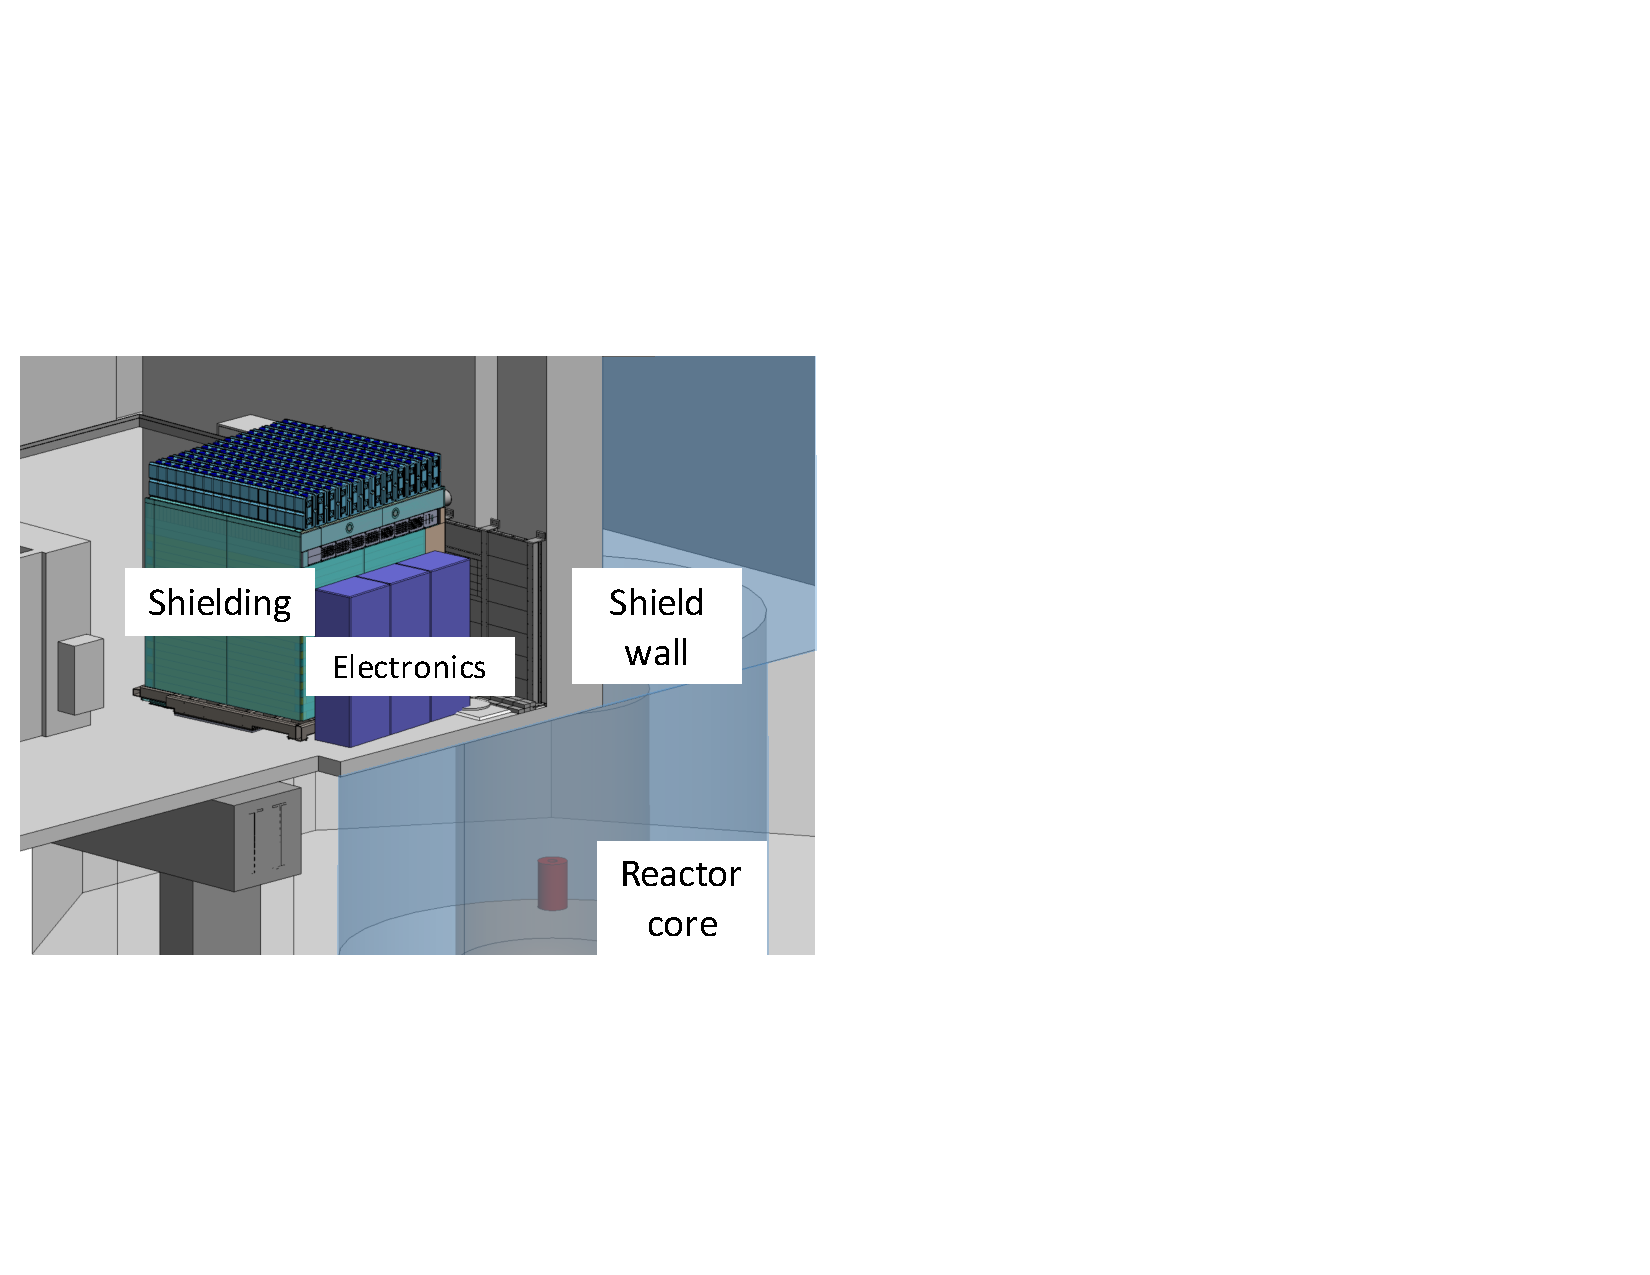
\includegraphics[width=0.5\linewidth]{tex/4-prospect-images/Shielding}
	\caption[Layout of PROSPECT at HFIR]{Layout of the PROSPECT experiment. The detector is installed in the HFIR Experiment Room next to the water pool and 5 m above the HFIR reactor core (red). The floor below contains multiple neutron beam-lines and scattering experiments.}
	\label{fig:shielding}
\end{figure}

\section{Design}

The PROSPECT antineutrino detector (AD) consists of a segmented inner detector filled with $^6$Li doped liquid scintillator (LiLS), contained in an acrylic and aluminum tank, and surrounded by layers of passive shielding. 
The active detector is made up of a 14  $\times$ 11 array of optically separated segments, viewed on each end by a photomultiplier tube (PMT) enclosed in an acrylic housing. 
The AD is placed with the segments parallel to the reactor pool wall, $\sim$7 m from the reactor core, and measures $\sim$3 m tall including all shielding. 
See Figure~\ref{fig:ad} for a schematic of the detector. 

\begin{figure}[t]
	\centering
	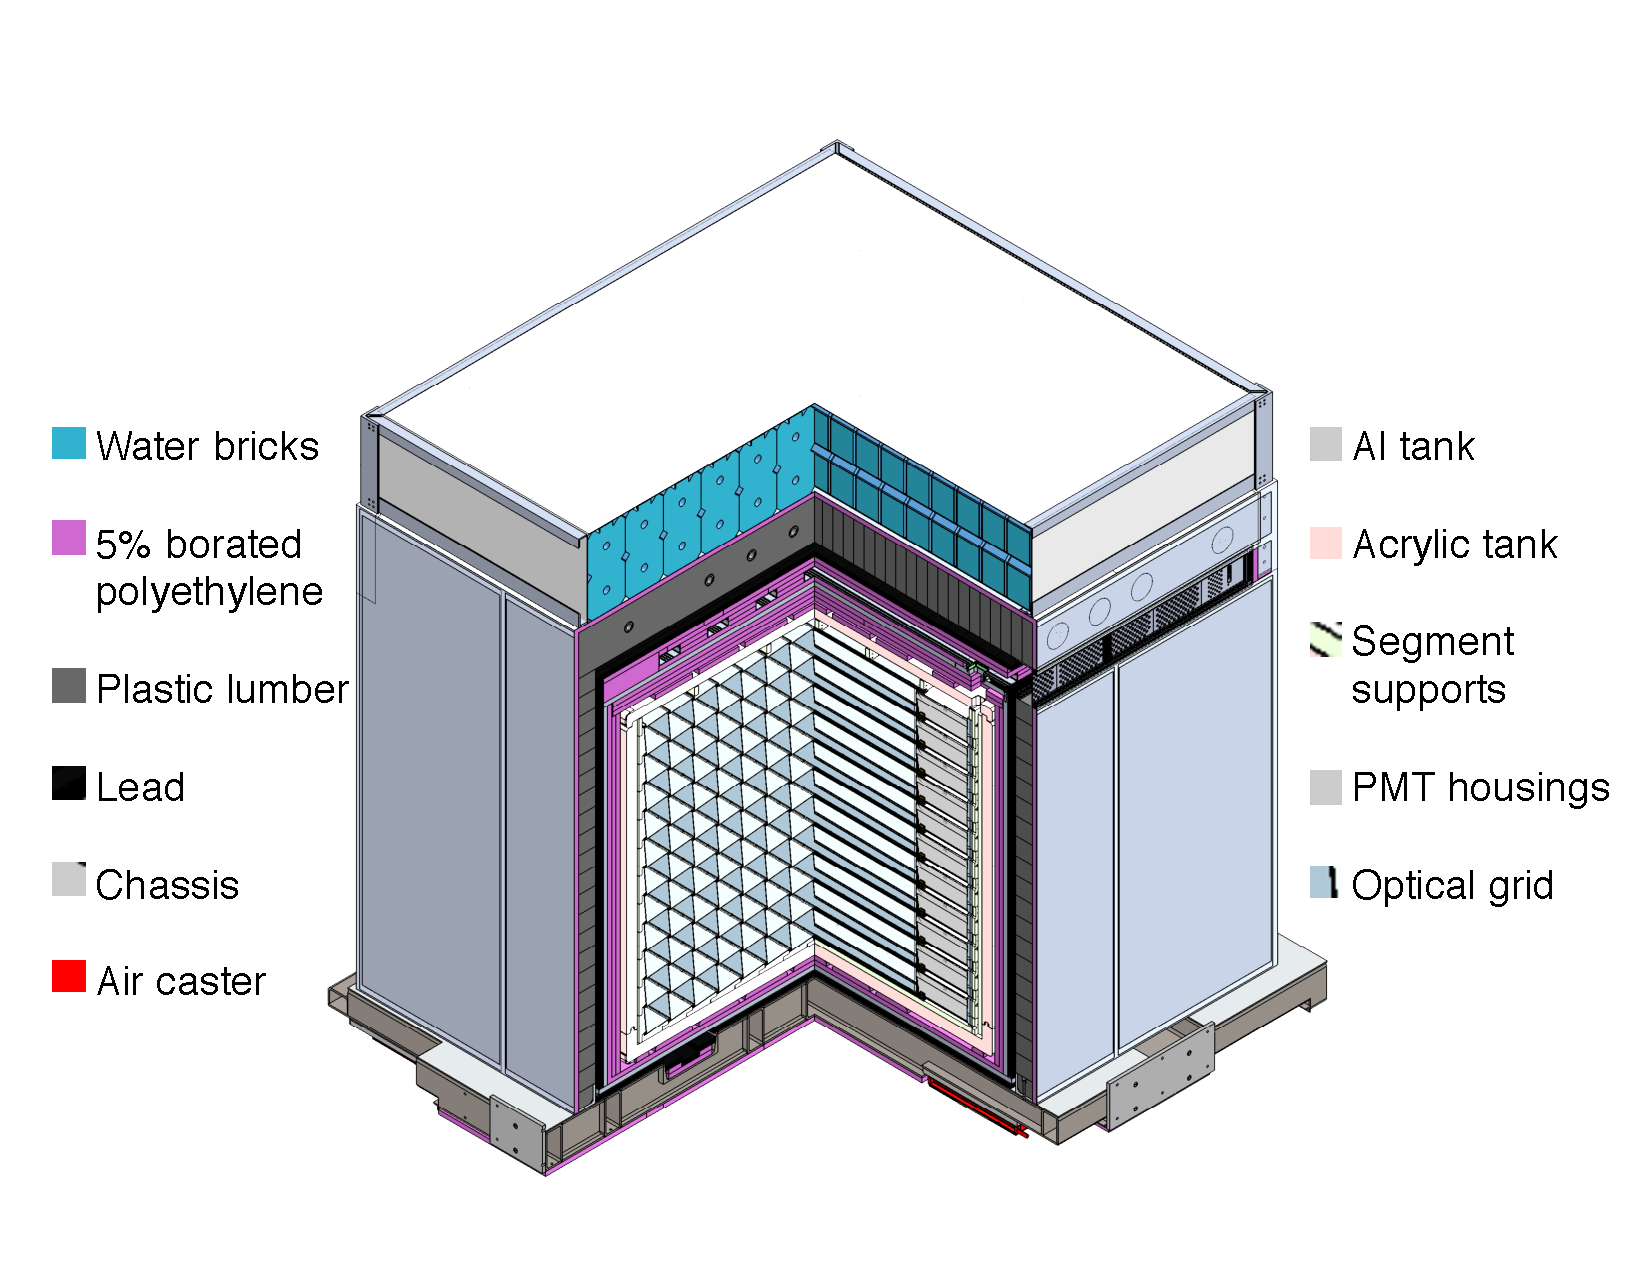
\includegraphics[width=0.8\linewidth]{tex/4-prospect-images/AD}
	\caption[Schematic of the PROSPECT detector]{A cutaway view of the PROSPECT detector, including the inner detector, outer containment vessels, and passive shielding.}
	\label{fig:ad}
\end{figure}

%===========================================================
\subsection{Active Detector} \label{sec:InnerDetector}

\subsubsection{PMT Housings}

A total of 308 PMTs are installed in the AD; 240 Hamamatsu R6594 SEL PMTs used in the inner segments (fiducial volume) and 68 ADIT Electron Tubes 9372KB PMTs used in the outer segments as shown in Figure~\ref{fig:adcrosssection}.
Each PMT is mounted inside a rectangular acrylic housing facing a clear 144-mm-square front window constructed from ultraviolet transmitting (UVT) acrylic, allowing them to exist inside of the LiLS. 
Conical reflectors were installed at the face of the housing to improve light collection efficiency in the corners. 
The housing is filled with optical grade mineral oil and sealed with an O-ring and a 32-mm-thick back plug. 
For a detailed drawing of the PMT housing module see Figure~\ref{fig:pmthousing}.
For more information on the PMT housing design and construction see Ref.\cite{LongNIM}.

\begin{figure}[h]
	\centering
	\begin{minipage}[t]{0.48\linewidth}
		\centering
		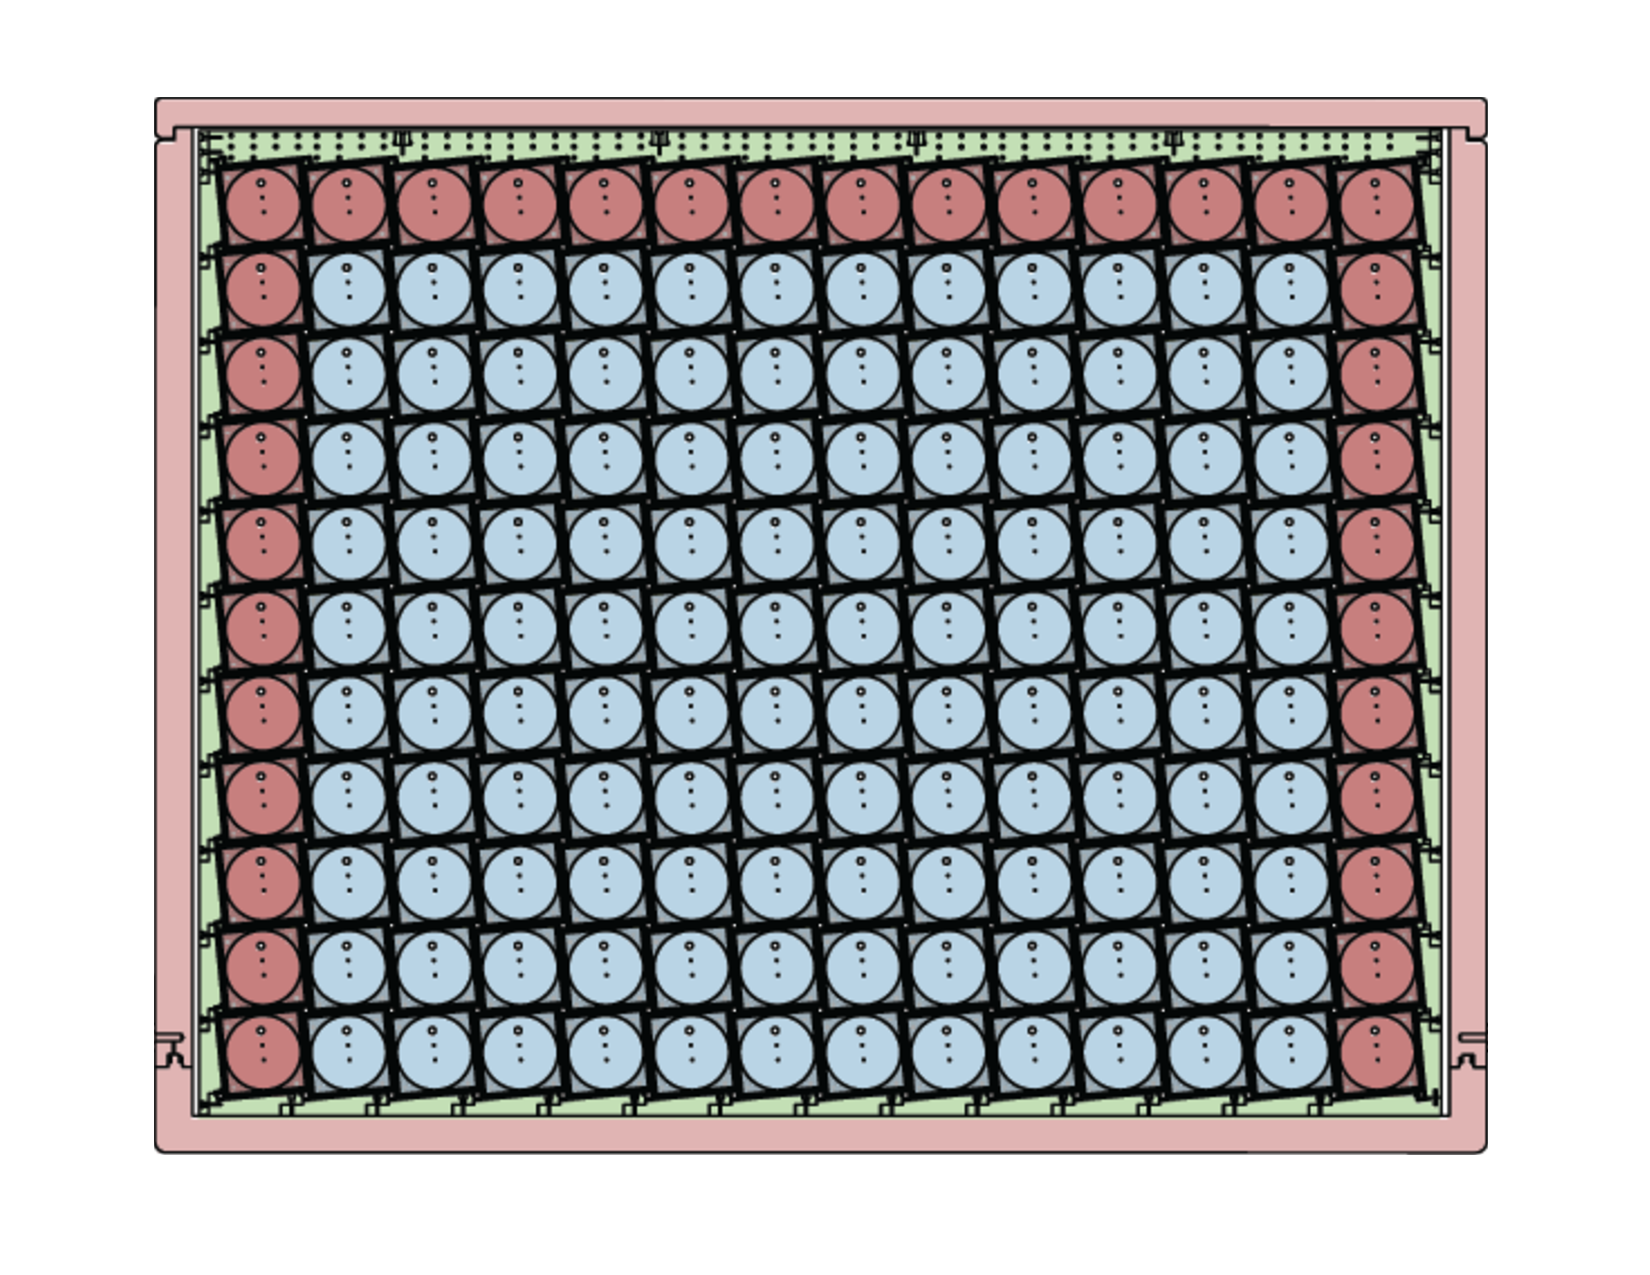
\includegraphics[width=0.95\linewidth]{tex/4-prospect-images/ADCrossSection}
		\caption[Cross-section of inner detector]{A cross-section of the inner AD showing 68 ET PMTs (red) in the outer columns and top row and 240 Hamamatsu PMTs (blue) in the remaining segments.}
		\label{fig:adcrosssection}
	\end{minipage}
	\begin{minipage}[t]{0.48\linewidth}
		\centering
		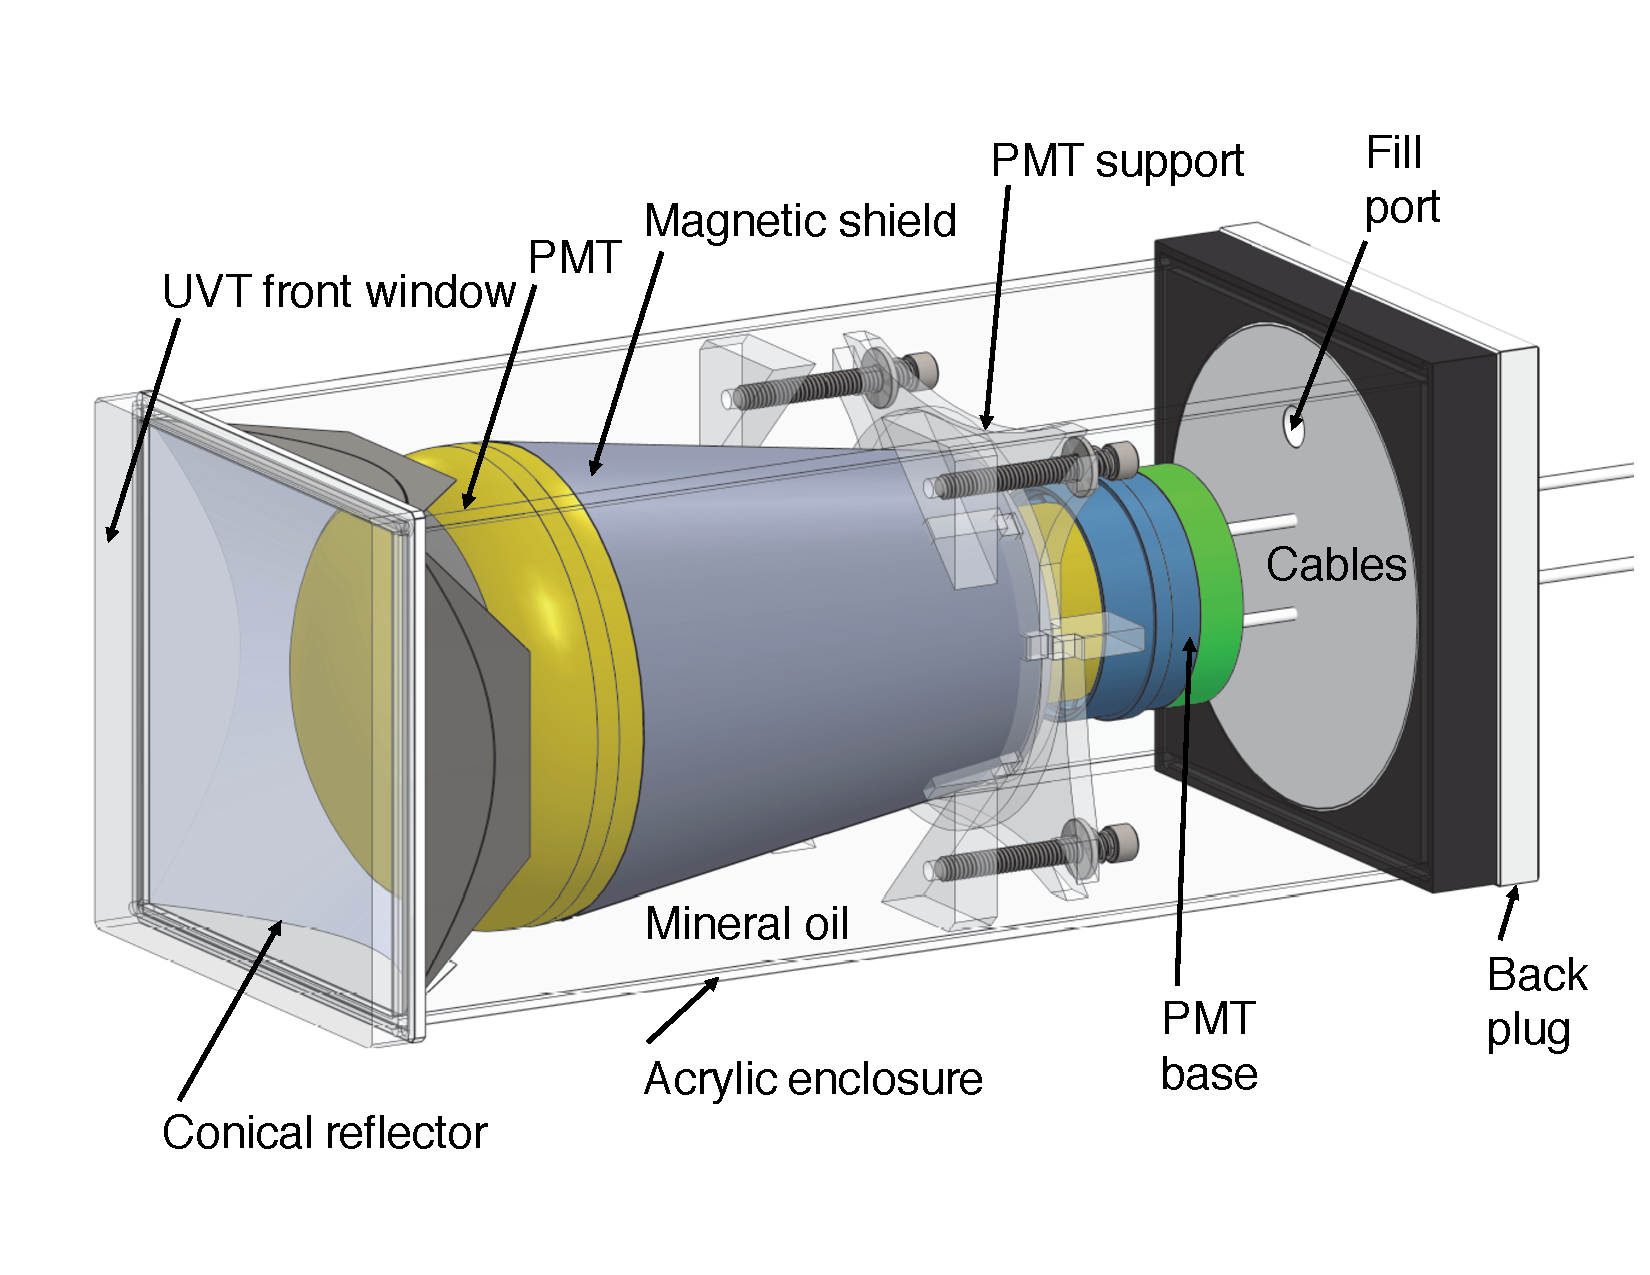
\includegraphics[width=0.95\linewidth]{tex/4-prospect-images/PMTHousing}
		\caption[PMT housing module]{A PMT housing module.}
		\label{fig:pmthousing}
	\end{minipage}
\end{figure}


\subsubsection{Optical Grid}

The active volume of the detector, measuring 2.045 m wide $\times$ 1.607 m high $\times$ 1.176 m long, is separated into 154 optically separated long segments with a 0.145 m $\times$ 0.145 m square cross-sectional area. 
The optical grid that creates the individual segments consists of low-mass, highly specularly reflective optical separators held in position by white 3D-printed support rods. 
The optical separators (reflectors) are composed of a carbon fiber backbone covered on both sides with adhesive-backed 3M DF2000MA specularly reflecting film, an optically clear adhesive film, and a thin surface layer of fluorinated ethylene propylene (FEP) film.
Two types of pinwheel shaped support rods were produced and strung on acrylic rods to grip the reflectors and hold them in place and separate the PMT housings from each other.
The pinwheels were 3D printed using white-dyed 100-micron polylactic acid (PLA) filament and are pictured in Figure~\ref{fig:pinwheels}.
For more details on the fabrication of the optical grid see Ref.\cite{Ashenfelter:2019lbf}.

Each segment contains a PMT housing at each end and four reflectors held in place by pinwheel rods that extend from one PMT to the other, as show in Figure~\ref{fig:fullsegment}.
The front windows of the PMT housings protrude $\sim$ 1 cm into the optical grid, minimizing cross-talk 
between segments. 
Figure~\ref{fig:rowassembly} shows the assembly of the top row of the detector, demonstrating the placement of the housings and optical grid. 


\begin{figure}[]
	\centering
	\begin{minipage}[t]{0.4\linewidth}
		\centering
		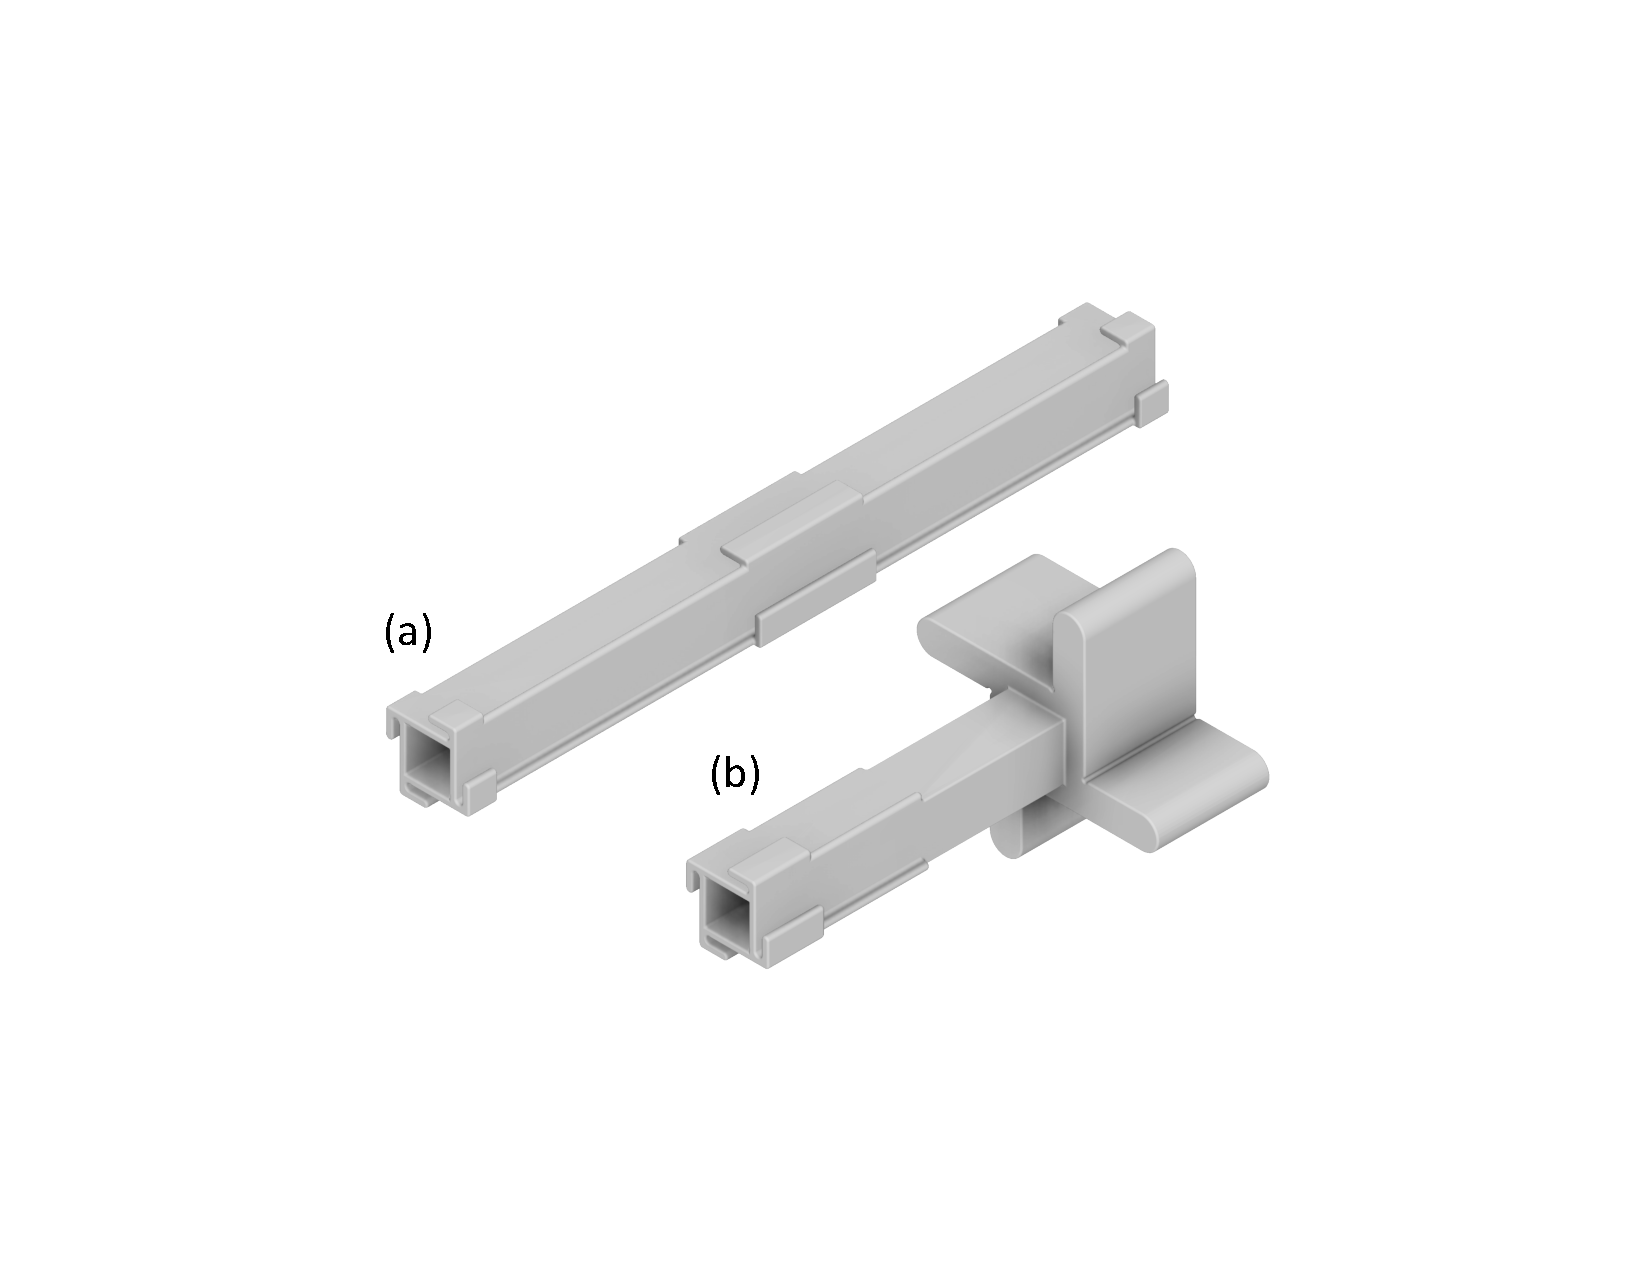
\includegraphics[width=0.8\linewidth]{tex/4-prospect-images/Pinwheels}
		\caption[Pinwheels]{Representative pinwheel types. (a) Central pinwheel - Three tabs per side hold the optical
		separator in place. (b) End pinwheel - spacer arms separate the PMT housing bodies and support the
		pinwheel string.}
		\label{fig:pinwheels}
	\end{minipage}
	\begin{minipage}[t]{0.48\linewidth}
		\centering
		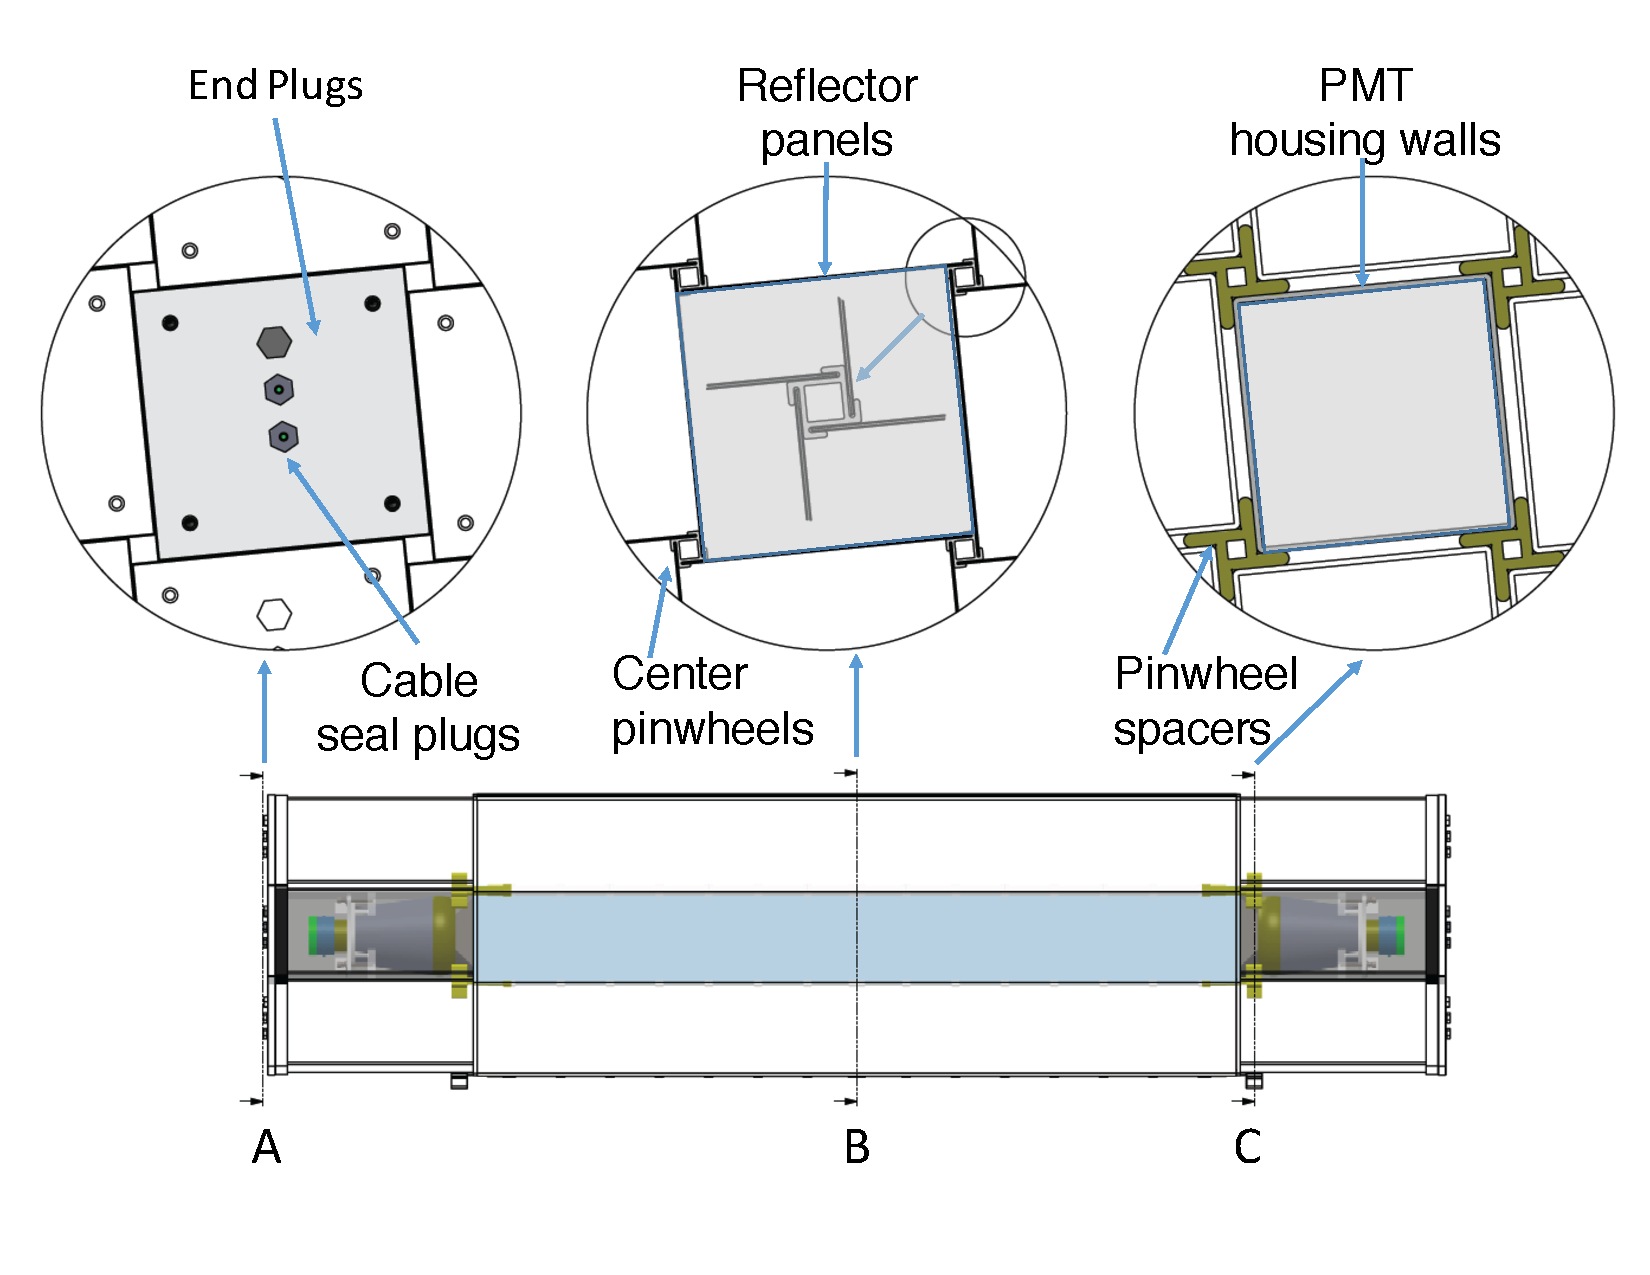
\includegraphics[width=0.98\linewidth]{tex/4-prospect-images/FullSegment}
		\caption[Schematic of a segment]{Three complete segments, including PMT housings at each end with reflectors kept in in place between segments by pinwheel rods.}
		\label{fig:fullsegment}
	\end{minipage}
\end{figure}

\begin{figure}[]
	\centering
	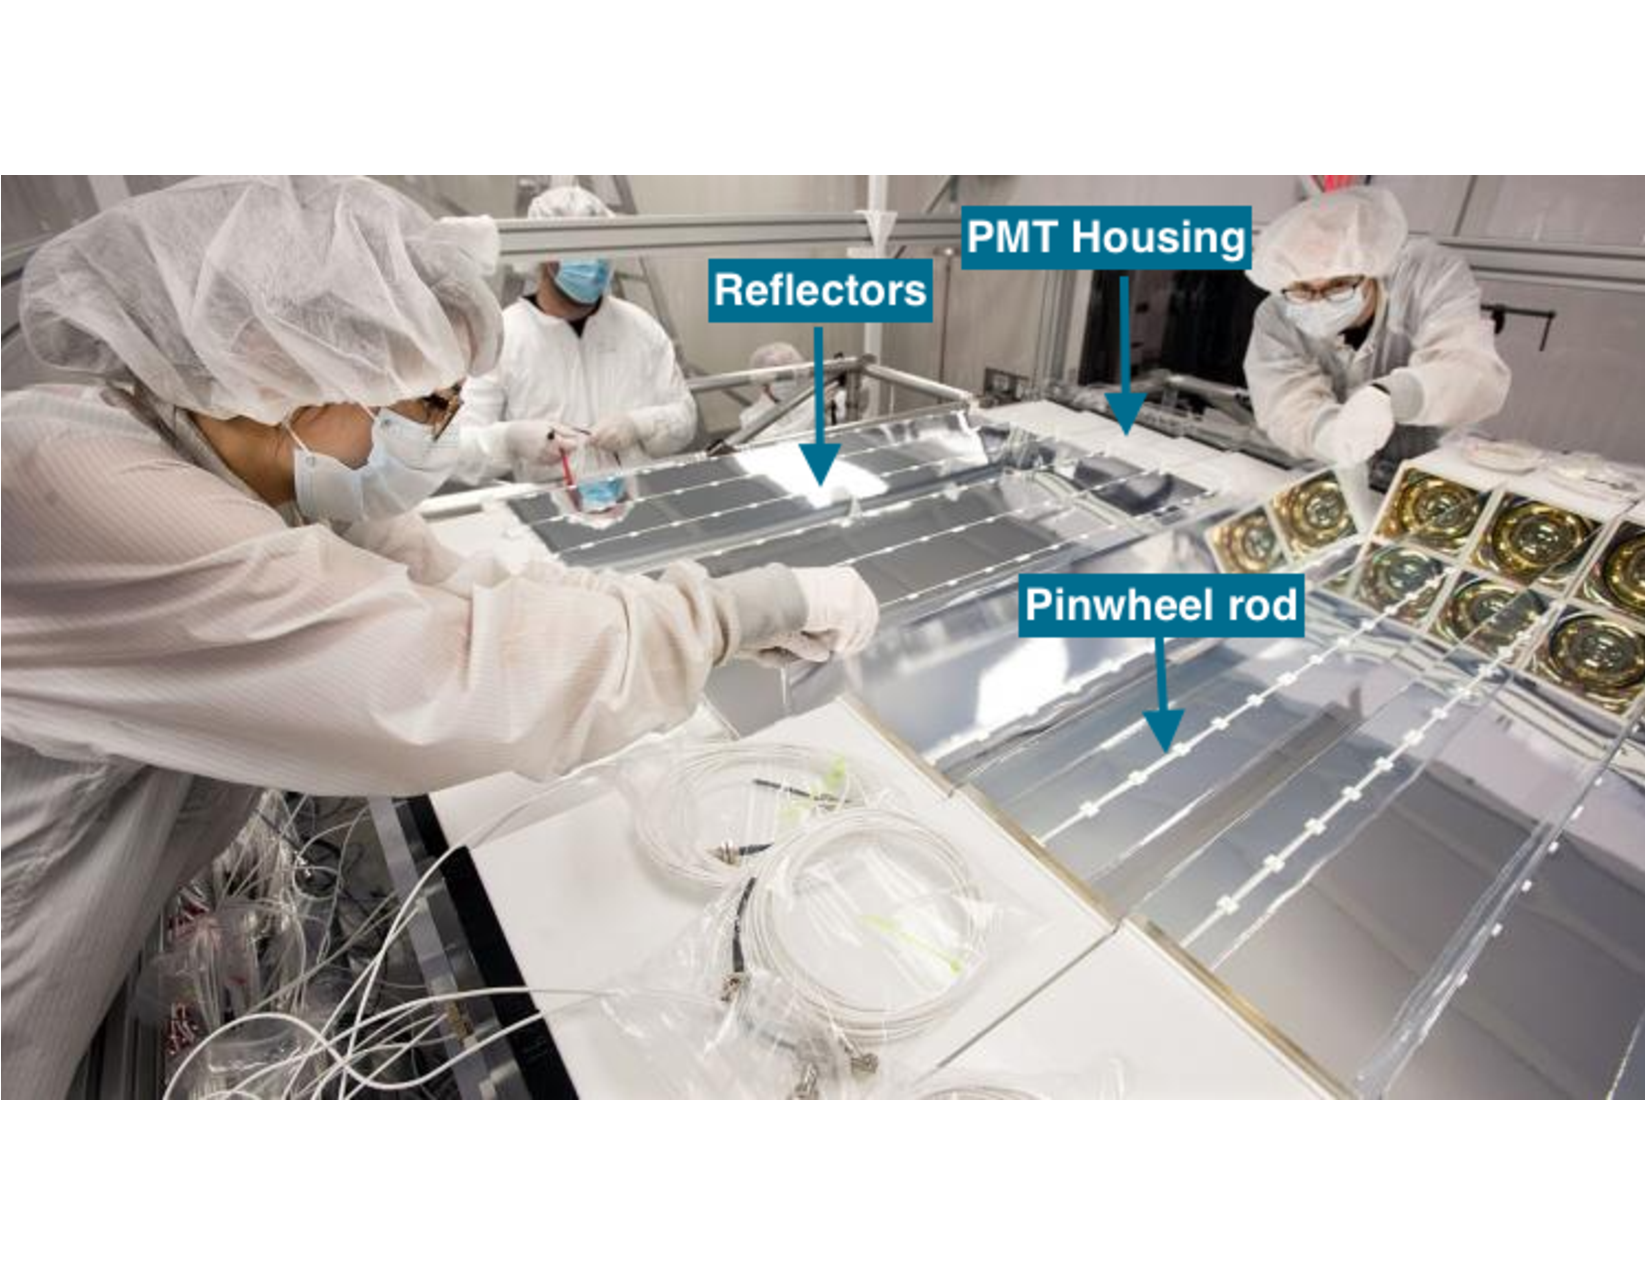
\includegraphics[width=0.7\linewidth]{tex/4-prospect-images/RowAssembly}
	\caption[Construction of a row]{Assembly of the top row of the PROSPECT AD, demonstrating the placement of the PMT housings and optical grid.}
	\label{fig:rowassembly}
\end{figure}


\subsubsection{Segment Supports}

While the optical grid creates the inner volume segmentation, acrylic segment supports hold the total volume in place and determine the size of the active volume.
A slab of ship-lap style acrylic underneath the bottom row of segments position them at a 5.5$^{\circ}$ tilt with a 0.146 m pitch.
Horizontal planks are screwed onto the backs of the PMT housings and attach together along the sides of the volume, while side walls constrain the outer pinwheel rows. 
Baffles at the top of the detector tie the four surrounding walls together and keep the top reflector layer in place. 
The construction of the inner detector, including all segment supports, allows the liquid scintillator to flow around all objects and therefore fill the whole space.
For a photograph of the constructed inner detector see Figure~\ref{fig:completeddetector}.
\begin{figure}[h]
	\centering
	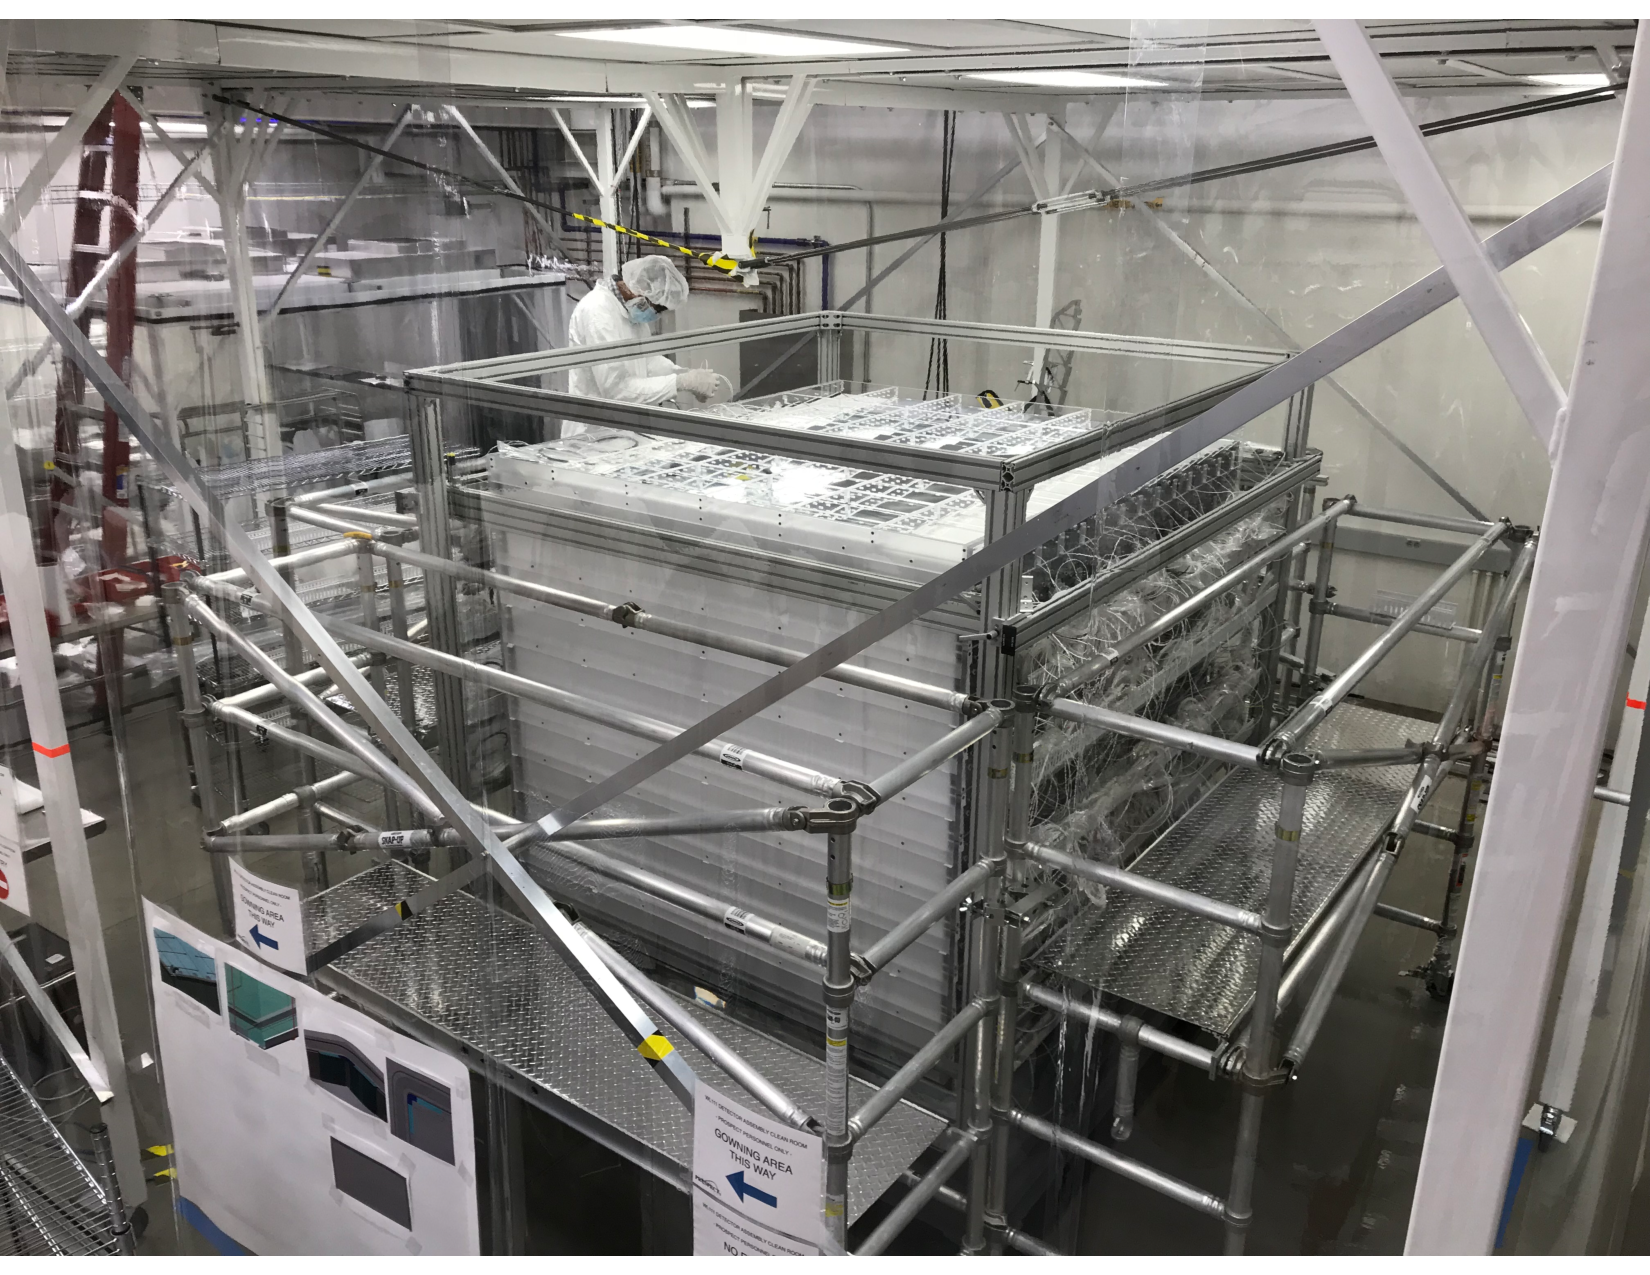
\includegraphics[width=0.7\linewidth]{tex/4-prospect-images/CompletedDetector}
	\caption[Completed inner detector]{A photograph of the constructed inner detector.}
	\label{fig:completeddetector}
\end{figure}


\subsubsection{Radioactive Calibration System}

The radioactive calibration system is designed to measure and calibrate the energy and position response of the detector as well as to study topological effects. 
It does this my moving radioactive sources through a system of tubes routed throughout the active detector, the positions of which are pictured in Figure~\ref{fig:adcalibrationtubes}.
PROSPECT deploys $^{137}$Cs, $^{22}$Na, $^{60}$Co, $^{252}$Cf, and an AmBe source, the features of which are listed in Table~\ref{tab:Sources}.

Each source is encapsulated in a small aluminum cylinder, about 12 mm long, and then connected to a timing belt as pictured in Figure~\ref{fig:sourcecapsule}.
The timing belts are placed in source tubes that run along the length of the segments and are controlled by motors mounted outside of the detector volume. 
For more information on the construction of the calibration system see Ref.\cite{Ashenfelter:2019jzp}.

PROSPECT also makes use of intrinsic radioactive sources for calibration and monitoring of detector characteristics. 
Two of these are colloquially known as ``BiPo" decays, and they arise from the $^{212}$Bi $\rightarrow ^{212}$Po + $\beta \rightarrow ^{208}$Pb + $\alpha$ and $^{214}$Bi $\rightarrow ^{214}$Po + $\beta \rightarrow ^{210}$Pb + $\alpha$ decay chains which stem from naturally occurring $^{232}$Th ($t_{1/2}$ = 14 Gyr) and $^{238}$U ($t_{1/2}$ = 4.5 Gyr), respectively.
Along with these, a solution of $^{227}$Ac was added to the liquid scintillator to provide a source of ``RnPo" decays from the chain $^{219}$Rn $\rightarrow ^{215}$Po + $\alpha \rightarrow ^{211}$Pb + $\alpha$.
Further details on the motivation and results from adding actinium will be discussed in Chapter~\ref{ch:Ac}.


\begin{table}[t]
\begin{tabular}{|c|c|c|c|c|}
	\hline 
	\bf{Source} & \bf{Decay} & \bf{$\gamma$ Energy [MeV]} & Purpose & Rate \\ 
	\hline 
	$^{137}$Cs & $\beta^-$ & 0.662 & segment comparison & 0.1 $\mu$C \\ 
	\hline 
	$^{22}$Na & $\beta^+$ & 2$\times$ 0.511, 1.275 & positron, edge effects & 0.1 $\mu$C \\ 
	\hline 
	$^{60}$Co & $\beta^-$ & 1.173, 1.332 & energy scale & 0.1 $\mu$C \\ 
	\hline 
	$^{252}$Cf & n (fisson) & 2.223 (n-H capture) & neutron response & 866 n/s \\ 
	\hline 
	AmBe & n & 4.4 & neutron response & 70 n/s \\ 
	\hline 
\end{tabular} 
\caption[Calibration sources]{Calibration sources and their properties.}
\label{tab:Sources}
\end{table}

\begin{figure}[h]
	\centering
	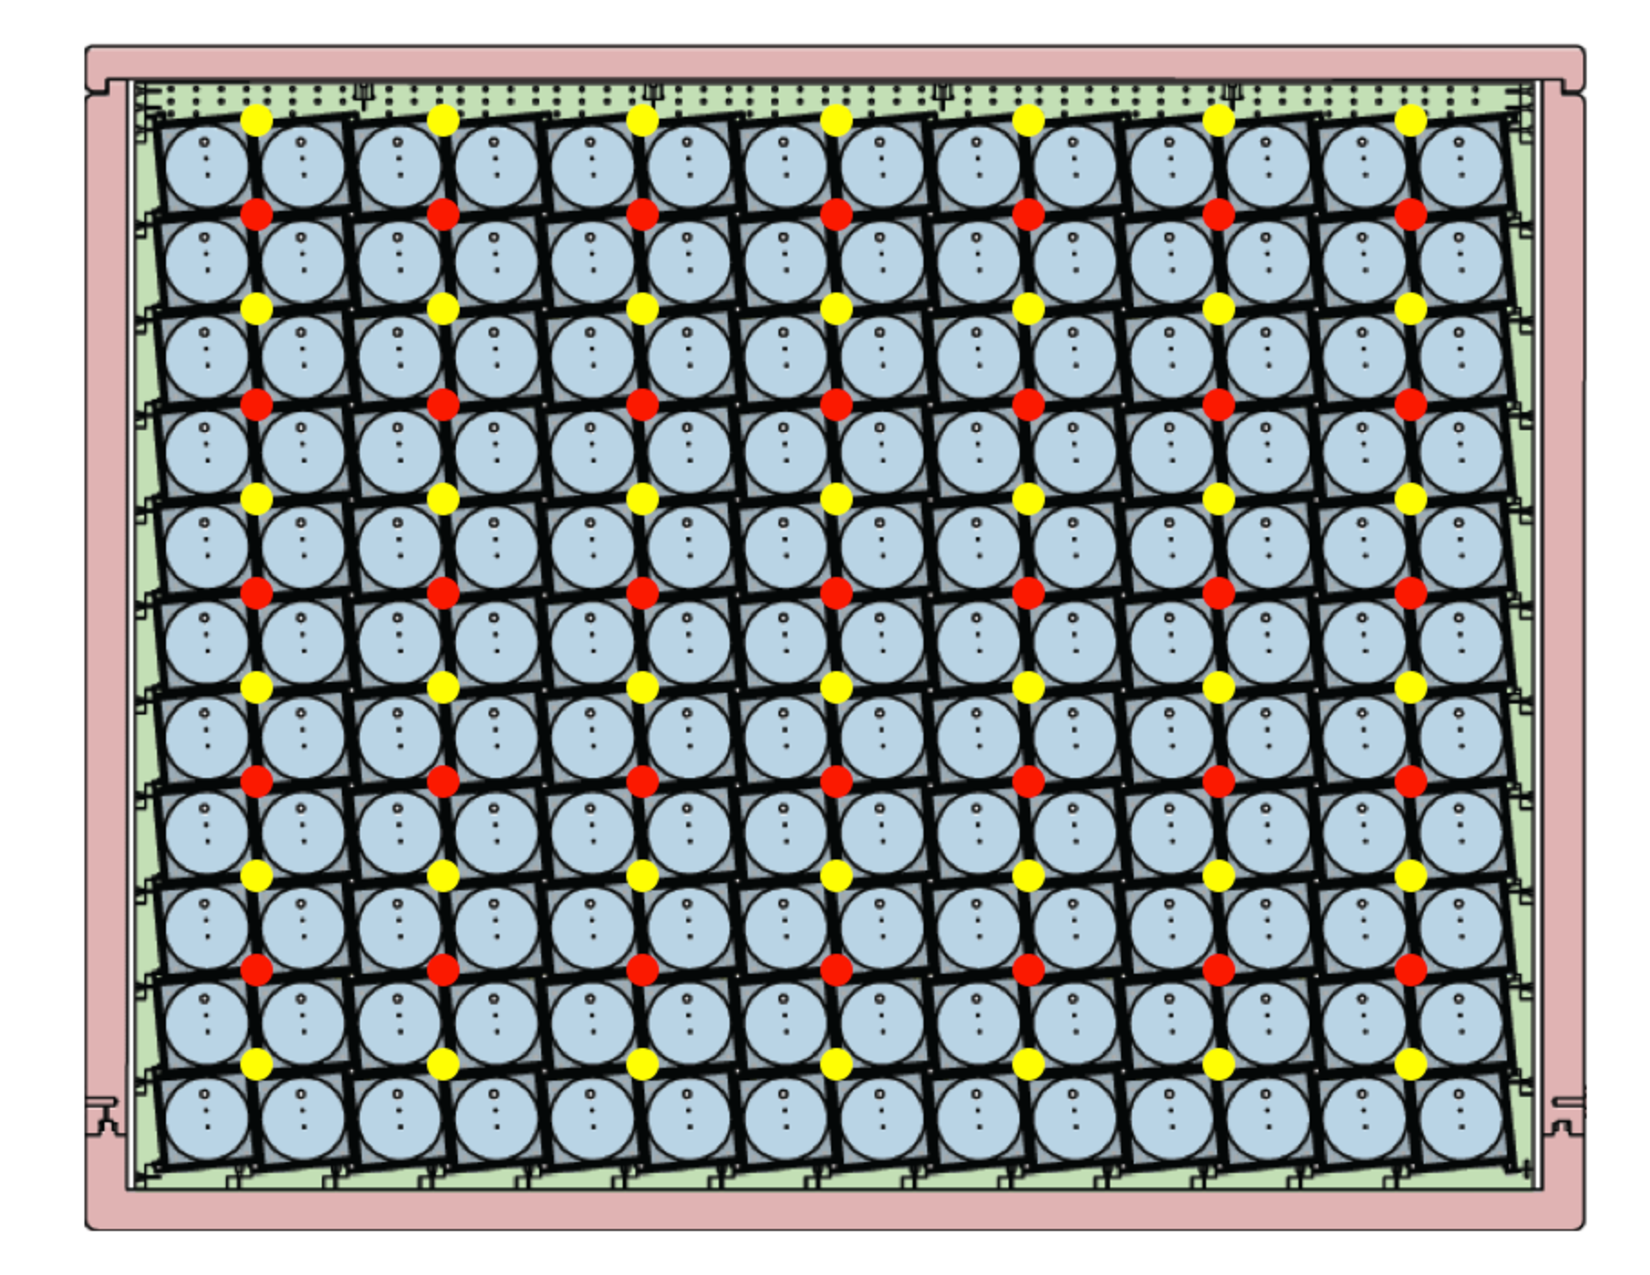
\includegraphics[width=0.7\linewidth]{tex/4-prospect-images/ADCalibrationTubes}
	\caption[Source tube positions]{Location of the source tubes (red) routed through the active detector volume.}
	\label{fig:adcalibrationtubes}
\end{figure}

\begin{figure}[h]
	\centering
	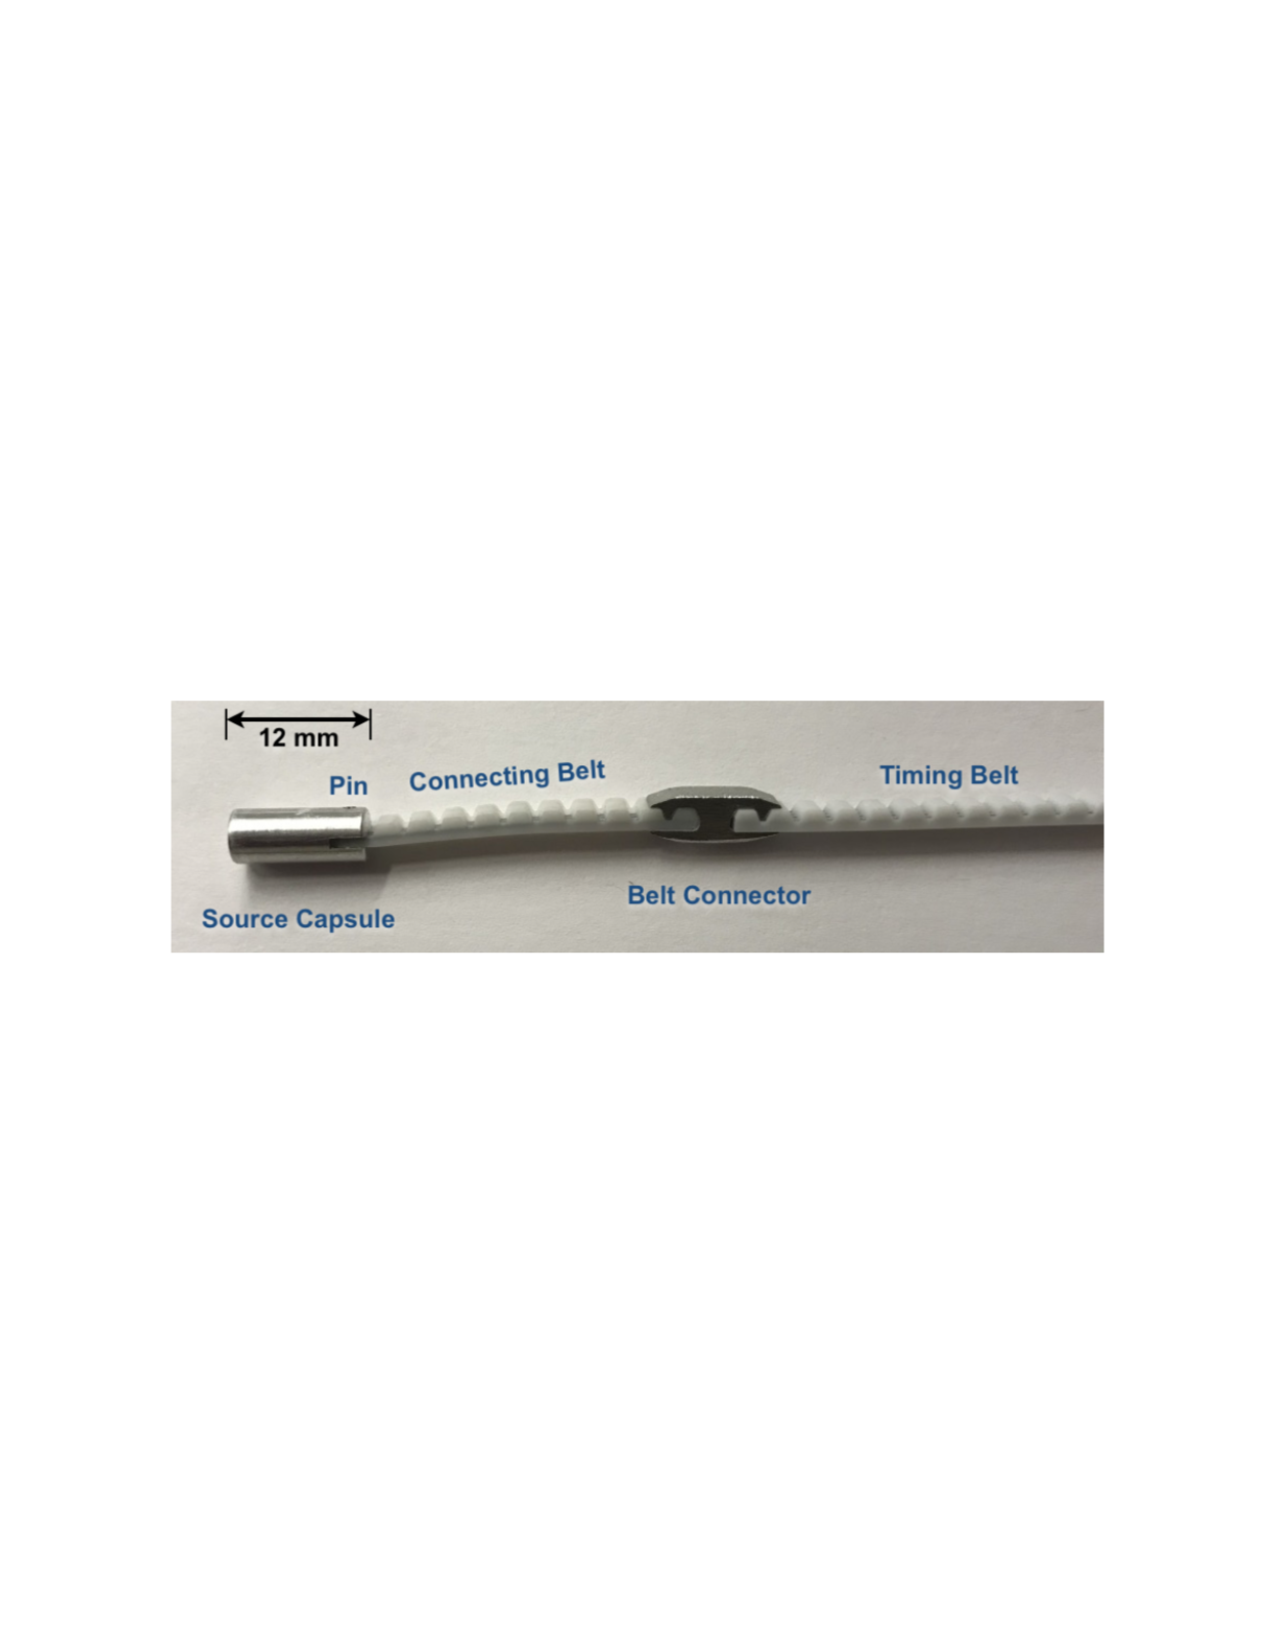
\includegraphics[width=0.7\linewidth]{tex/4-prospect-images/SourceCapsule}
	\caption[Source capsule on timing belt]{An example of a source capsule attached to the timing belt.}
	\label{fig:sourcecapsule}
\end{figure}



\subsubsection{Liquid Scintillator}

The liquid scintillator (LS) used in PROSPECT needed to accomplish two goals: (i) provide very good pulse shape discrimination (PSD) for sufficient background rejection of fast neutrons and ambient gammas and (ii) have high light yield in order to obtain good energy resolution. 
The LS also needed to remain stable over time and non-flammable according to facility requirements. 
In order to accomplish these tasks PROSPECT developed a novel lithium-doped liquid scintillator (LiLS). 
$^6$Li was chosen as the doping agent due to it's high neutron capture cross section, which produces an $\alpha$ and a $^3$H with about 540 keV of visible energy in the scintillator. 
These particles are also spatially localized, which is necessary for the compact detector size of PROSPECT.

The LiLS was created by adding a surfactant to the base LS which allowed the addition of a $^6$LiCl solution to obtain a final doping of 0.082\%$\pm$0.001\% by mass. 
The combination of the surfactant and chloride solution forms a thermodynamically stable micro emulsion, ensuring material uniformity and allowing the addition of an actinide chloride solution ($^{227}$Ac). 
A total of 5,040 liters were produced and stored in 28 separate drums. 
One drum was doped with a $^{227}$Ac chloride solution. 
For more information on the fabrication of the LiLS see Ref.\cite{Ashenfelter:2019iqj}.

Prior to filling the detector, all drums of LiLS were pumped into an ISO tank storage container. 
Nitrogen was then bubbled through the liquid for ten days to sufficiently mix together the solution.
Samples were taken from each barrel and from the mixed solution in the ISO tank with a Shimadzu UV-Vis spectrometer, the results of which can be seen in Figure~\ref{fig:lils}.
4841 kg of LiLS was pumped into the ISO tank and a total of 4340 kg was then added to the detector. 
For more information on the process of filling the detector with the LiLS see Ref.\cite{LongNIM}.

\begin{figure}[h]
	\centering
	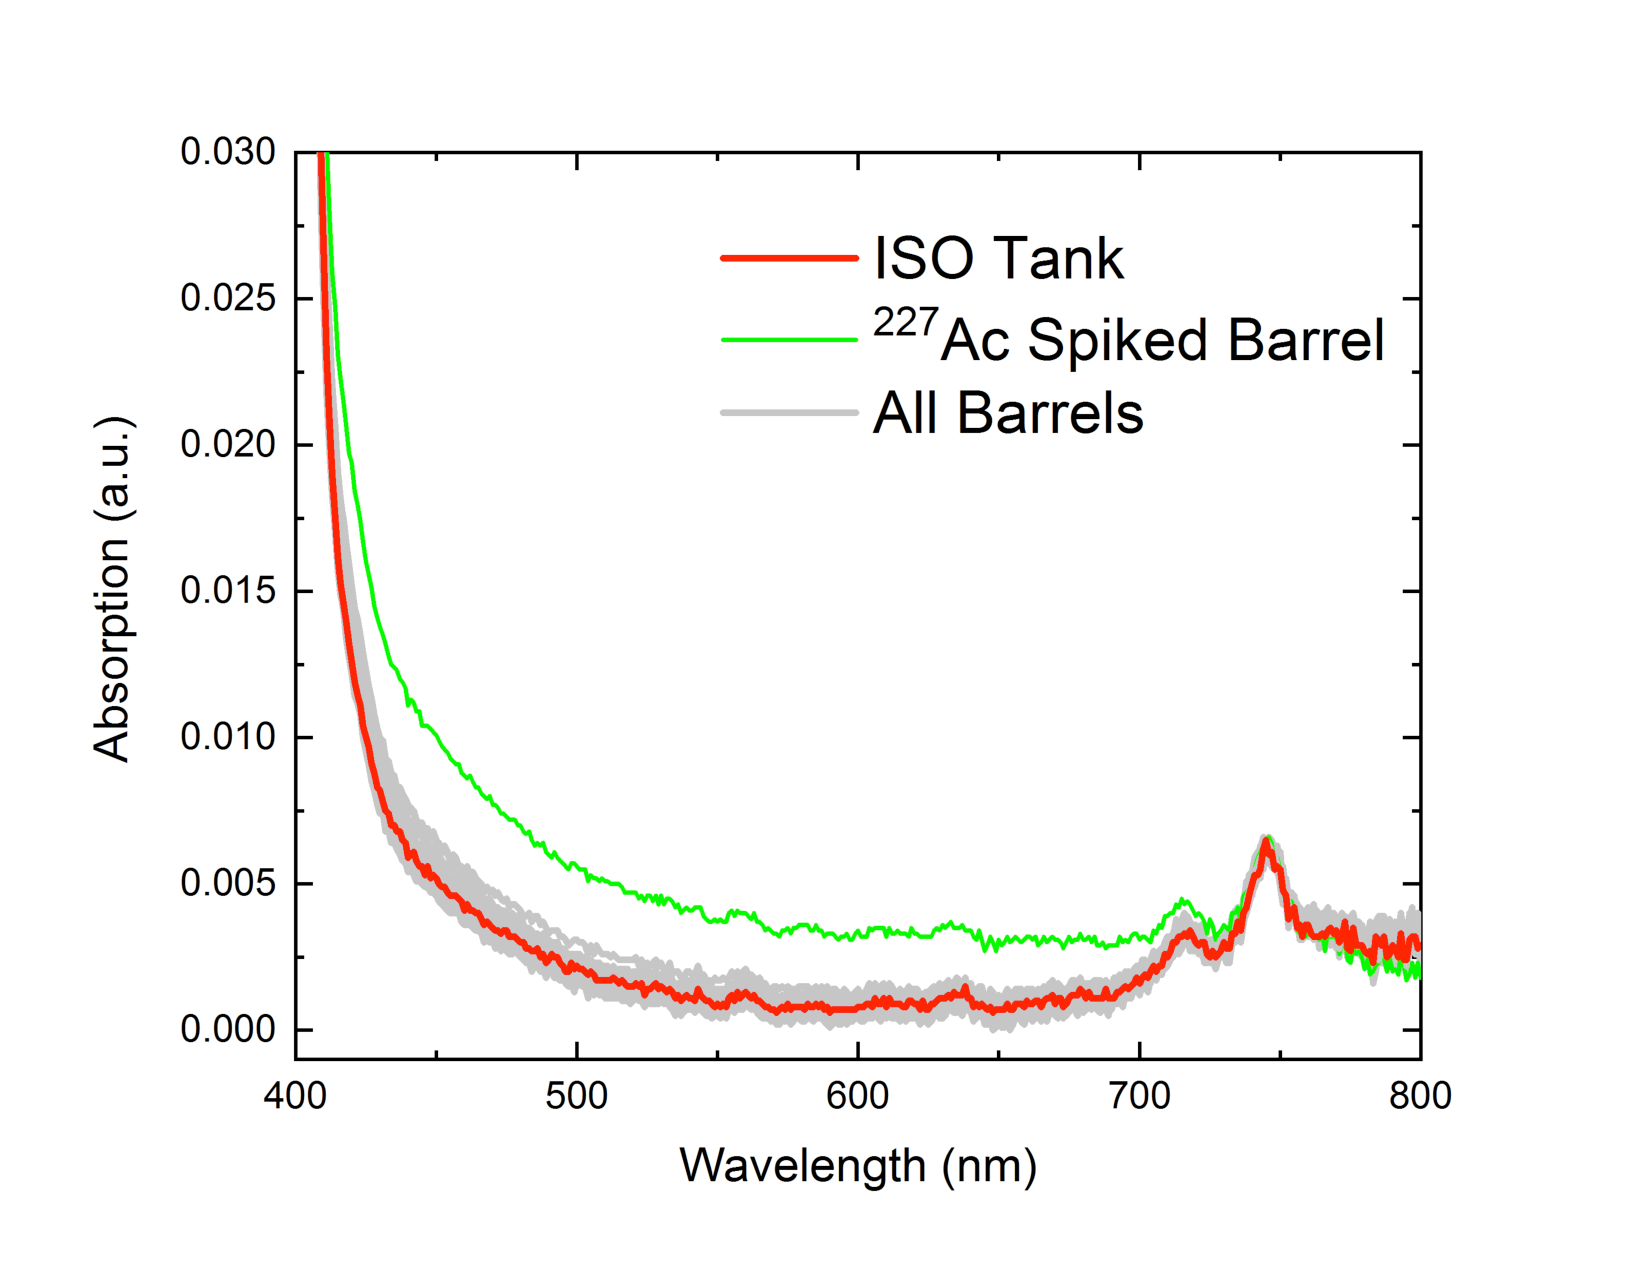
\includegraphics[width=0.6\linewidth]{tex/4-prospect-images/LiLS}
	\caption[LiLS UV-Vis absorption spectra]{UV-Vis absorption spectra of the 28 drums if LiLS (gray+green) added to the ISO tank. The only outlier is the $^{227}$Ac spiked barrel (green). The mixed sample (red) falls within the average of all individual barrels.}
	\label{fig:lils}
\end{figure}


%===========================================================
\subsection{Containment Vessels and Shielding} \label{sec:shielding}

The inner primary containment vessel is made of acrylic and holds all active detector components described in Section~\ref{sec:InnerDetector}. 
The acrylic tank was built as three separate parts, the base, vertical walls, and lid. 
The inner detector was assembled on the acrylic base. After its constructions the vertical walls were lowered onto the base and secured with a Viton seal at the base. 

The secondary containment vessel is made of aluminum and the top is sealed in order to control the gas environment around the detector.
The space between the aluminum and acrylic tanks is filled with sheets of borated polyethylene and demineralized water for absorption of thermal neutrons.

A lead layer of 0.025 m $\times$ 0.10 m $\times$ 0.30 m interlocking brick was stacked around the perimeter of the aluminum tank. 
Rows of 0.10 m $\times$ 0.10 m recycled polyethylene lumber were stacked on each other log cabin style and then placed around the lead layer.
Polyethylene lumber was also used to create roof beams on top of the log cabin walls.
The entire surface was then covered with a 0.025 m thick layer of borated polyethylene and thin aluminum sheets. 
To complete the passive shielding an array of water bricks were added to the top of the assembly. 
For a schematic of the entire construction see Figure~\ref{fig:ad}.



%===========================================================
%===========================================================
\section{Data Acquisition System} \label{sec:DAQ}

In order to perform pulse discrimination analysis of LiLS signals PROSPECT uses commercial Waveform Digitizer Modules (WFDs).
A total of twenty-one CAEN V1725 WFD modules, operated in two Weiner 6023VME crates, are used to readout the 308 PMTs. 
Readout and control of the WFD modules is performed by two individual PCs, which are run by a control PC. 
A single Phillips Scientific 757D NIM Fan-In/Fan-Out module operated in a NIM bin is used for trigger signal distribution.
A diagram of this system can be seen in Figure~\ref{fig:daq}.

Acquisition of waveforms 148 samples long by all WFD channels is triggered if both PMTs in any segment exceed a signal level of 50 ADC counts above baseline ($\sim$100 keV) within a 64 ns coincidence window.  
Acquired samples from each WFD are only recorded to disk if they exceed a threshold limit of 20 ADC counts above baseline ($\sim$40 keV). 
These are labeled the segment and Zero Length Encoding (ZLE) thresholds and allow the acceptance of low energy events while maintaining a manageable data collection. 
For more information of the data acquisition system and data rates see Ref.~\cite{LongNIM}.

\begin{figure}[h]
	\centering
	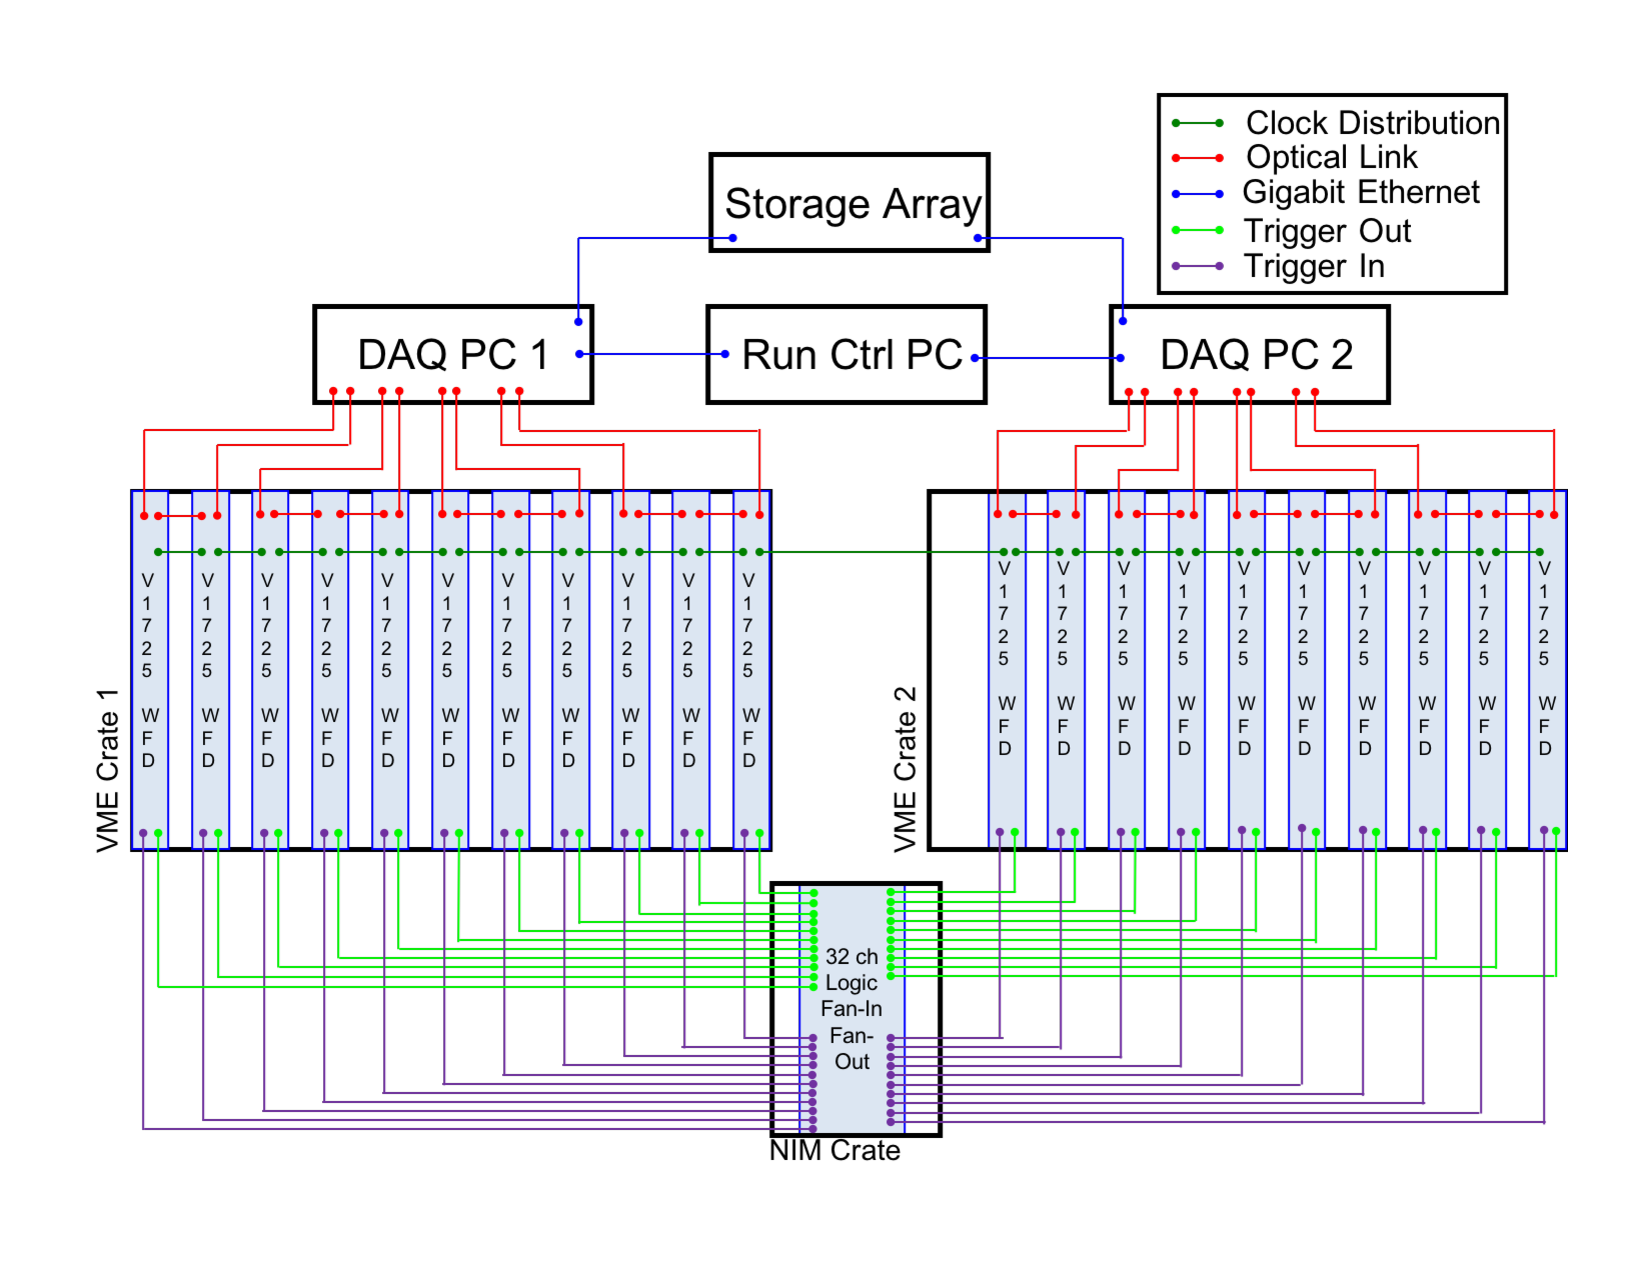
\includegraphics[width=0.7\linewidth]{tex/4-prospect-images/DAQ}
	\caption[DAQ schematic]{Diagram of the data acquisition system.}
	\label{fig:daq}
\end{figure}


